\chapter{Introduction}
\label{sec:intro}
\chaptermark{Introduction}

To present the ideas outlined in the abstract of this document it is necessary to start with a collection of definitions. Some will be given here, while others will need to be taken from references or outside sources. The natural starting point of this discussion is to present a useful example of symmetries that are observed in the world and how these are classified in physics. Next, a basic discussion of field theory and scattering amplitudes will be presented. From these examples, the discussion will expand to a categorization of the particles, fields, and symmetries that make up The Standard Model of Particle Physics. Equipped with these definitions and ideas we will investigate some specific features of this model, including an introduction of Electroweak symmetry breaking, discrete symmetries, and then limitations of the current model.

\section{Symmetries in Physics}
\label{sec:Symmetries}

Symmetry is one of, if not the, most important features in the physics of the natural world. As we pull together the various pieces needed to present the state of the art in particle physics we will define multiple symmetries that exist in nature and how we use them to test our current and hypothetical models.

\subsection{Noether's Theorem}
\label{sec:Noether}

To begin, let us define the \textit{symmetry group} of the system, $G$, as the local group that transforms solutions into other solutions.\footnote{We have not formally defined a group in this document, for an interested reader see \cite{Armstrong:1988,Miller:1972,Oliver:1993,Tung:1985}} If $x$ is a solution and $g$ is a group element then $ g \cdot x$ will also be a solution. In Physics, the solutions that we consider are ones that maximize or minimize the action:  

\begin{equation}
\label{eq:action}
\mathcal{S} = \int d^{4}x{\mathscr{L}}.
\end{equation}

Where the integrand, $\mathscr{L}$, is the \textit{Lagrangian} of the system, $\mathscr{L} = T - V$. The symbols $T$ and $V$ are used for the kinetic and potential energy respectively. So a symmetry group of a physical system would be the set of transformations that leave the Lagrangian invariant. This concept became one of most important in physics after Emmy Noether proved that these symmetries of the action correspond to conserved quantities that do not change as the system evolves \cite{Noether:1918zz}.

\subsection{Angular Momentum and the Rotation Group}
\label{sec:AngularMomentum}

To demonstrate the importance of Noether's Theorem let us consider the group of rotations in 3 dimensional space, the special orthogonal group in 3 dimensions, $\mathrm{SO}(3)$. Given any unit vector $\hat{\textbf{n}}$ a rotation about this vector by an angle $\psi$ is denoted by $R_{\hat{\textbf{n}}}(\psi)$. Here we will use the Euler Angles to parameterize $R$, where the rotations about the $(x,y,z)$ axis are given by $(\alpha, \beta, \gamma)$ respectively. It will also be useful to note that performing a rotation $R_{1}$ followed by another rotation $R_{2}$ is equivalent to a single rotation $R_{3}$, or that the set of rotations is closed.

\begin{figure}
\label{fig:Euler}
\begin{center}
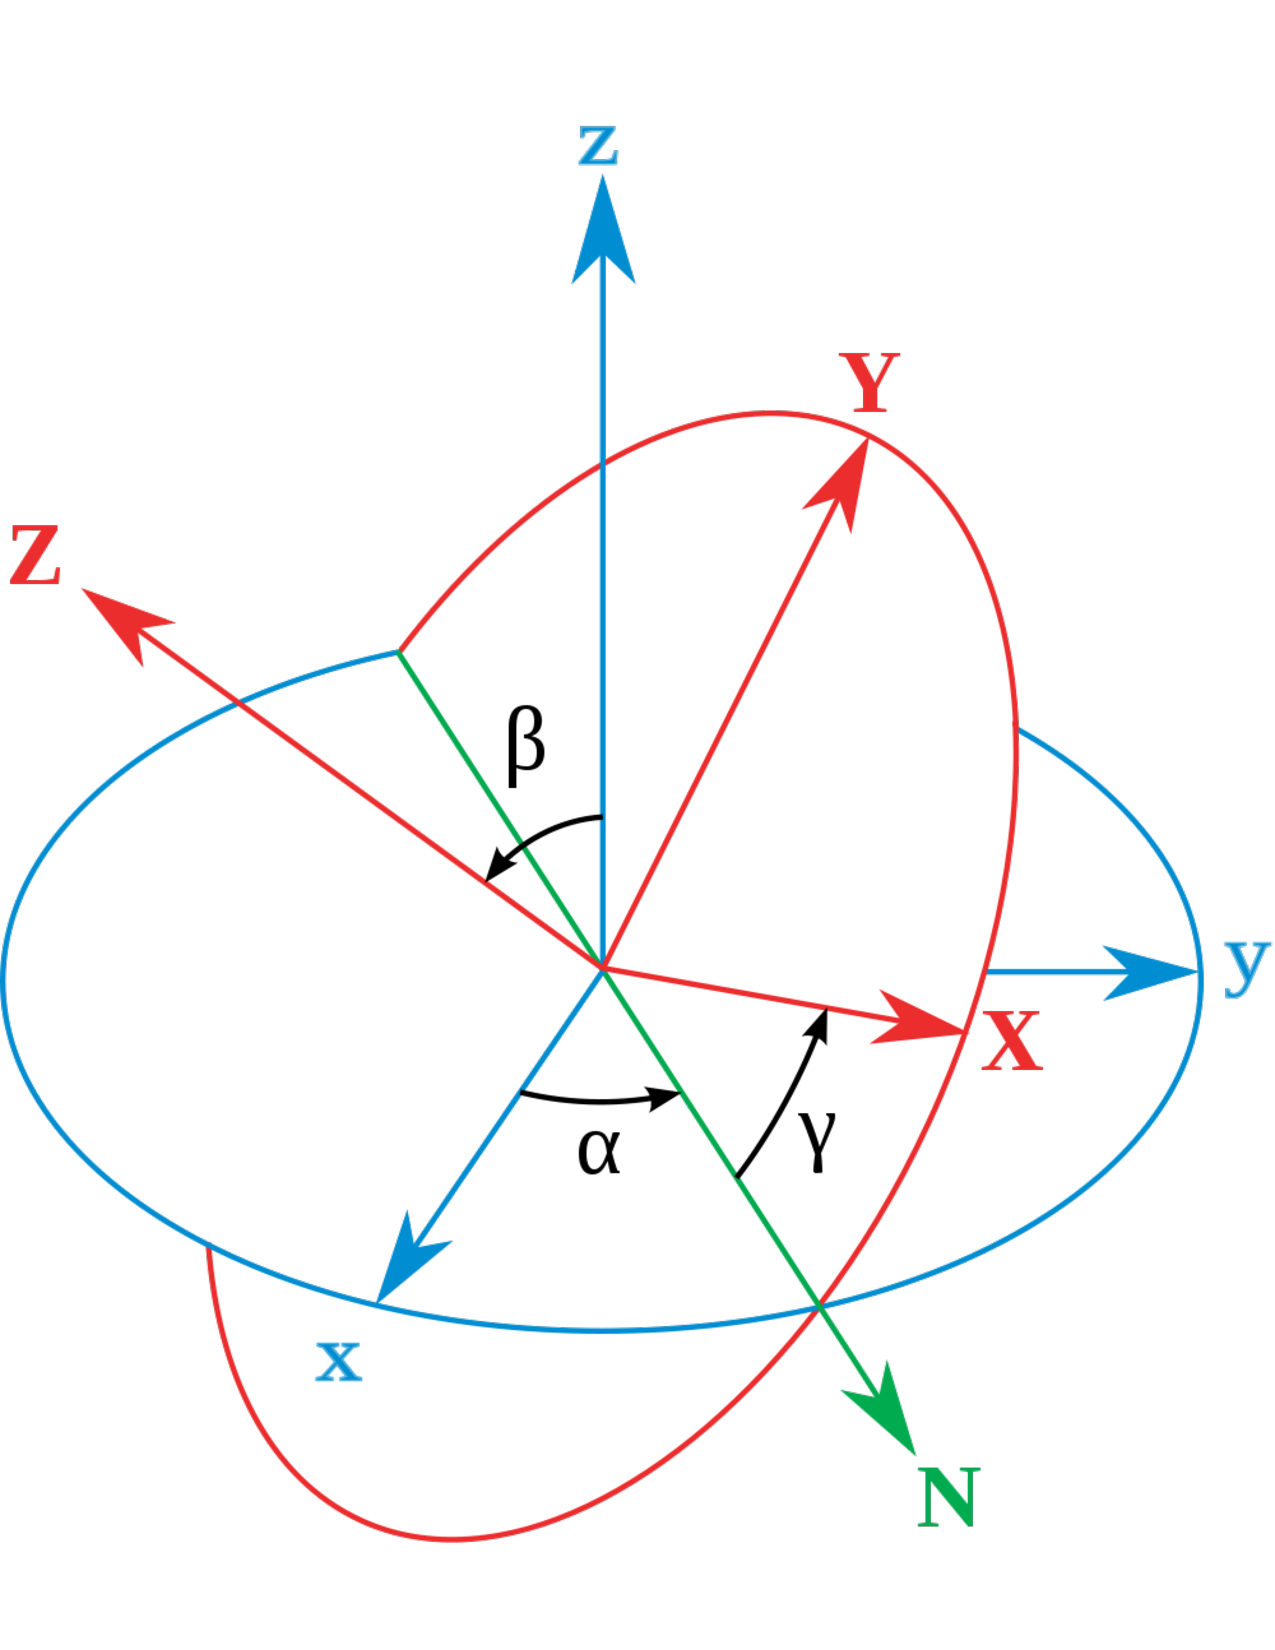
\includegraphics[width=0.5\linewidth]{Introduction/Euler.pdf}
\caption{Euler angles for three dimensional Cartesian coordinates.\cite{wiki:Euler}}
\end{center}
\end{figure}


A arbitrary rotation $R(\alpha, \beta, \gamma)$ can be decomposed into rotations about the fixed axes, $R(\alpha, \beta, \gamma) = R_{x}(\alpha)R_{y}(\beta)R_{z}(\gamma)$. Figure \ref{fig:Euler} shows these angles for the transformation of vector $N$ from $(x,y,z)$ to $(X,Y,Z)$. At this point is is useful to express the rotations $R_{x,y,z}$ in terms of their matrix formulation, Equations \ref{eq:Second},\ref{eq:Third},\ref{eq:Fourth}. Where the angle of rotation must satisfy $0 \leq \psi \leq 2\pi$.

\begin{equation}
\label{eq:Second}
R_{z}(\psi) = \left( \begin{array}{ccc}
cos\psi & -sin\psi & 0 \\
sin\psi & cos\psi & 0 \\
0 & 0 & 1 \end{array} \right)
\end{equation}

\begin{equation}
\label{eq:Third}
R_{y}(\psi) = \left( \begin{array}{ccc}
cos\psi & 0 & sin\psi \\
0 & 1 & 0 \\
-sin\psi & 0 & cos\psi \end{array} \right)
\end{equation}

\begin{equation}
\label{eq:Fourth}
R_{x}(\psi) = \left( \begin{array}{ccc}
1 & 0 & 0 \\
0 & cos\psi & -sin\psi \\
0 & sin\psi & cos\psi \end{array} \right) 
\end{equation}

In this formulation it is clear to see that a vector along the $z$-axis direction will be left unchanged due to a $R_{z}$ rotation. More generally, we can apply Noether's Theorem when the Lagrangian for a physical system does not depend on infinitesimal rotations about the any axis, $\mathscr{L}-\mathscr{L}(\delta\alpha,\delta\beta,\delta\gamma) = 0$. This symmetry corresponds to the classical conservation of angular momentum, $\mathrm{J}$ when the Lagrangian has spherical symmetry. This symmetry will become important as we discuss the kinematics of the particles we use to study new discoveries.

\subsection{Inherent Spin and $\mathrm{SU}(2)$}
\label{sec:SU2}

If one fixes a direction in equations \ref{eq:Second}, \ref{eq:Third}, and \ref{eq:Fourth} then the rotations about that direction will form a subgroup of $\mathrm{SO}(3)$. This becomes clear when you consider the closure, identity, and inverse group axioms for the subset of rotations $R_{z}$. Specifically, the subgroup is isomorphic to the special unitary group of rotations in two dimensions, $\mathrm{SU}(2)$. One way to write this new transformation is: 

\begin{equation}
\label{eq:Dim2}
R(\phi) = \left( \begin{array}{cc}
cos\phi & -sin\phi \\
sin\phi & cos\phi \end{array} \right)
\end{equation}

The simplest way to represent a group is to find the elements that all other elements of the group can be made from. To find these elements for $\mathrm{SU}(2)$ start with equation \ref{eq:Dim2} and consider an infinitesimal rotation $d\phi$. Since $R(\phi)$ is differentiable one can derive an equation to write all possible rotations in terms of the operator matrix $\mathrm{J}$ which we will call the \textit{generator} of $\mathrm{SU}(2)$. Explicitly, $R(\phi)$ can be written as:

\begin{equation}
\label{eq:generator}
R(\phi) = e^{-i \frac{\phi}{2} \mathrm{J}},
\end{equation}

where $\mathrm{J}_{i} = \sigma_{i}$ and $\sigma_{i}$ is one of the Pauli matrices:

\begin{equation}
\label{eq:Pauli}
\sigma_{1} = \begin{pmatrix}
    0 & 1\\
    1 & 0
  \end{pmatrix}, \sigma_{2} = \begin{pmatrix}
    0 & -i\\
    i & 0
  \end{pmatrix}, \sigma_{3} = \begin{pmatrix}
    1 & 0\\
    0 & -1
  \end{pmatrix}
  \end{equation}


In this formulation $R(\phi)$ operates on states that are linear combinations of \textit{two-component spinors} given by equation \ref{eq:spinors}. These spinor eigenstates have an inherent conserved spin with energy $\hbar/2$. 

\begin{equation}
\label{eq:spinors}
\chi_{+} = \begin{pmatrix} 1 \\ 0 \end{pmatrix}, \chi_{-} = \begin{pmatrix} 0\\1\end{pmatrix}
\end{equation}

Fermions states can be expressed as linear combinations of these two component spinors, but we will find it more useful to transform the basis so that they can be rewritten in terms of the two component spinors $\psi_{R}$ (right-handed) and $\psi_{L}$ (left-handed) that are eigenstates of the parity transformation\footnote{As position transforms from $\vec{x} \to -\vec{x}$ the momentum transforms as $\vec{p} \to -\vec{p}$}.

\begin{equation}
\label{eq:TwoRandL}
\psi = \begin{pmatrix} \psi_{R} \\ \psi_{L} \end{pmatrix}
\end{equation}

These fermions and the group $\mathrm{SU}(2)$ will be two of the major building blocks that are used when we discuss the Standard Model of particle physics. Before we describe this model we will take some time to discuss Scattering Amplitudes.

\section{Scattering Amplitudes}
\label{sec:Scattering}

Particle physics at its core is not very different from pre-school; we want to see what is inside of something but can't get our hands in the tiny spaces, so we smash it apart. The complexity that is swept under the rug in this statement is that we can map what is happening in these small spaces to what we observe using scattering amplitudes, which tell us the behavior of particles as they "break away" from the things we are trying to study. More generally, a scattering matrix tells us how a system of particles will evolve over time, either because of collisions between particles or other natural processes.

\subsection{Scattering Matrix}
\label{sec:Smatrix}

To explain how particle physics explains the evolution of a system over time, we will follow a procedure outlined in \cite{Maggiore5.1:2005}. Let us consider a set of particles with certain characteristics denoted $\ket{\psi}\left(t\right)$. The system at a time $t$ is given in Dirac notation\footnote{For a good explanation of Dirac notation see \cite{Schwabl:2002}}. We will denote the initial state of the system as $\ket{\psi_{i}} = \ket{\psi}\left(T_{i}\right)$, and the final state as $\bra{\psi_{f}} = \bra{\phi}\left(T_{f}\right)$. These states can be single or multiple particle states and typically quantities like momentum, spin, or helicity\footnote{Projection of spin onto momentum, $\vec{S}\cdot\hat{p}$} are used to specify them in this notation.

The evolution of a system from state $\ket{\psi_{i}}$ to $\bra{\psi_{f}}$ is given by
\begin{equation}
\label{eq:psiSpsi}
\bra{\psi_{f}}S\ket{\psi_{i}}.
\end{equation}
Where $S$ is a quantum mechanical operator associated with the scattering matrix. 

To give a concrete example you can consider a plane wave evolving over time. In this case, $S = e^{-iH\left(t-T_{i}\right)}$. For this explanation we have described the used a Hamiltonian\footnote{A Hamiltonian is simply the Legendre transformation of a Lagrangian.}, $H$, to describe the physical system instead of the Lagrangian. In this case, equation \ref{eq:psiSpsi} becomes

\begin{equation}
\label{eq:WaveSmatrix}
\bra{\psi_{f}}e^{-iH\left(T_{f}-T_{i}\right)}\ket{\psi_{i}}.
\end{equation}

In the limit that $T_{f} - T_{i} \to \infty$ the operator between the states is the \textit{scattering matrix} and maps some initial state to a final state at some other time. 

\subsection{Amplitudes and Feynman Diagrams}
\label{sec:Amplitudes}

Each of the states outlined in the previous section, $\ket{\psi}\left(t\right)$, will have specific properties. For example, the initial state may be in eigenstate $a$ for some commuting operator while the final state may be in eigenstate $b$ of the same operator. Then the evolution of the system from $\ket{a}$ to $\bra{b}$ will be through a specific \textit{matrix element}, $\mathcal{M}_{ab}$.

\begin{equation}
\label{eq:bSa}
\mathcal{M}_{ab} = \bra{b}S\ket{a}
\end{equation}

These matrix elements can be used to describe the evolution of the system through very specific transitions. The \textit{scattering amplitude}, $\mathrm{A}$ for a specific process can be computed as the modulus squared of the matrix element.
\begin{equation}
\label{eq:Amplitude}
\mathrm{A}_{ab} = \left|\mathcal{M}_{ab}\right|^{2} = \left|\bra{b}S\ket{a}\right|^{2}
\end{equation}

These amplitudes can also be expressed in a pictorial form, called \textit{Feynman diagrams}, that we will use extensively in this document. These diagrams are used to do the calculations through rules mapping vertex points, internal, and external lines to terms in the matrix element pieces.
  
%This is a sample equation:
%\begin{equation}
%\mathscr{L}_{EM} = \bar{\psi}\left(i\gamma^{\mu}(\partial_{\mu}+ieA_{\mu})-m\right)\psi - \frac{1}{4}F_{\mu\nu}F^{\mu\nu}.
%\label{eq:EMlagrangian}
%\end{equation}


To use a concrete example, we will describe the interaction of electrons through the electromagnetic interaction. The Lagrangian for two fermions\footnote{Defined in \ref{sec:SU2}} interacting elecgromagneticily is given by 
\begin{equation}
\label{eq:EMlagrangian}
\mathcal{L}_{EM} = \bar{\psi} \left(i\gamma^{\mu}\left(\delta_{\mu} + ieA_{\mu}\right) - m\right)\psi.
\end{equation}

In this equation, the electromagnetic interaction terms are represented by the vector potential, $A_{\mu}$ with $e$ as the coupling constant of the particle to the electromagnetic field. The $4 \times 4$ Dirac matrices $\gamma^{\mu}$ are defined by the $2 \times 2$ Identity matrix $\left(1\right)$ and the Pauli-matrices\footnote{Defined in \ref{sec:SU2}} we have already seen

\begin{equation}
\label{eq:GammaMatrix}
\gamma^{0} = \begin{pmatrix} 1 & 0 \\
					       0 & -1 \end{pmatrix},
\gamma^{i} = \begin{pmatrix} 0 & \sigma^{i} \\
                                               -\sigma^{i} & 0 \end{pmatrix}.
\end{equation}

In the amplitude notation this can be written as
\begin{equation}
\label{eq:eeScatteringAmpl}
A = \left|\bra{\psi_{1}\psi_{2}}e^{\bar{\psi}\left(i\gamma^{\mu}\left(\delta_{\mu} + ieA_{\mu}\right) - m\right)\psi}\ket{\psi_{1}\psi_{2}}\right|^{2}
\end{equation}

The equivalent representation lowest order terms of equation \ref{eq:EMlagrangian} as Feynman diagram will be Figure \ref{fig:eeScattering}. These diagrams can be used to quickly and simply represent complex interactions of particles and range from very simple, Figure \ref{fig:eeScattering}, to extremely complex, INSERT KU FEYNMAN DIAGRAM.

\begin{figure}
\begin{center}
\unitlength=1mm
\begin{fmffile}{eeScattering}

\begin{fmfgraph*}(40,30) \fmfpen{thick}
  \fmfleft{i1,i2} \fmfright{sp1,sp2}
  \fmf{fermion,label=$e^-$}{i1,v1,sp1} 
  \fmf{fermion,label=$e^-$}{i2,v2,sp2}
  \fmf{photon,label=$\gamma$}{v1,v2}
\end{fmfgraph*}

\end{fmffile}
\end{center}
\caption{Feynman diagram depicting electron-electron scattering via
the electromagnetic interaction.}
\label{fig:eeScattering}
\end{figure}

In this example we can see the properties of another group that will be important for the Standard Model. The electromagnetic interaction requires $\mathrm{U}(1)$ gauge symmetry. The conserved quantity for this group is the electric charge of the fermion, given by $e$ in the equations above. Now that we have introduced many of the pieces we need we will discuss the Standard Model of particle physics

\section{The Standard Model}
AND SO IT BEGINS!

%This is a sample table:

%\begin{table}
%\begin{center}
%\begin{tabular}{l|c|c|c|c}
%\hline 
%\hline
%particle & Q  & $T_3$ & $Y_W$ & colored \\ \hline \hline
%$e_L$, $\mu_L$, $\tau_L$  & -1 & -1/2   &  -1 &  no \\ 
%$e_R$, $\mu_R$, $\tau_R$  & -1 & 0      &  -2 &  no \\ 
%$\nu_L$  & 0   & 1/2 & -1 & no \\ 
%$u_L$, $c_L$, $b_L$    & 2/3 & 1/2  & 1/3& yes \\ 
%$u_R$, $c_R$, $b_R$    & 2/3 & 0  & 4/3& yes \\ 
%$d_L$, $s_L$, $t_L$    & -1/3& -1/2 & 1/3& yes \\ 
%$d_R$, $s_R$, $t_R$    & -1/3& 0 & -2/3& yes \\
%H        & 0   & 1/2  & -- & no \\
%W        & 1   & 1    & -- & no \\
%Z        & 0   & --   & -- & no \\
%$\gamma$ & 0   & --   & -- & no \\
%gluon    & 0   & 0    & 0  & yes \\
%\hline
%\end{tabular}
%\end{center}
%\caption{List of SM particles and their charges. 
%Q represents the charge of the $SU(1)_{em}$ gauge symmetry,
%$T_3$ the broken SU(2) gauge symmetry, and $Y_W$ the broken 
%U(1) gauge symmetry.}
%\label{table:SMcharges}
%\end{table}
